\section{Experiments and results}
\label{sec:experiments-results}

To determine how good our framework is, we compare it against an
adaptation of the well known heterogeneous bin packing solution as
discussed by Teodor et al.~\cite{tcra11}. They adapt the well-known
\textit{Best First Decreasing (BFD)} heuristic, which works only for
homogeneous bins, to form the \textit{Adapted BFD (A-BFD)} heuristic
which works for heterogeneous bins. We have chosen to compare our
framework against a bin-packing heuristic, because it is a well known
fact that the optimal solution for a partitioning problem is NP hard,
one cannot find optimal solutions for large processing
architectures. Heuristic bin packing solutions have given good results
in the general case~\cite{ecof78}. Comparing with the heterogeneous bin
packing heuristic allows us to gauge the effectiveness of our algorithm
against a standard effective technique.

\subsection{Heterogeneous Bin Packing}

Let $\mathcal{I}$ be the items to be accommodated into the bins and let
$\mathcal{K}$ be the set of bins available.  From the standpoint of the
mapping problem, $\mathcal{I}$ refers to the set of
\mbox{application-tasks ($|V_t|$)} and $\mathcal{K}$ refers to the PEs
($|V_r|$). Similar to the Knapsack problem~\cite{sski08}, by which A-BFD
is inspired, each element $i \in \mathcal{I},\ \mathcal{K}$ has two
constraints on them represented by \mbox{$c_i$ (cost)} and $V_i$
(volume).

\textit{A-BFD} proceeds to sort $\mathcal{I}$ according to
non-increasing order of their volume and sorts $\mathcal{K}$ according
to non-increasing order of the ratio $c_i/V_i$. Then, it proceeds to
allocate items from $\mathcal{I}$ into best bins $b \in \mathcal{S}$. A
``best" bin, i.e., the bin with maximum free space, is defined as the
bin volume minus the sum of volumes of the items loaded into
it.

The post pass in \textit{A-BFD} chooses every bin that has atleast one
item allocated to it and tries to find an empty bin, that has a higher
or equal volume than the allocated volume on the chosen bin but also has
a lower cost. If it finds such an empty bin, then it transfers all the
items allocated to the chosen bin to the newly found empty bin which is
cheaper. One of the main advantages of\ \textit{A-BFD} is that it is
very fast with a best case complexity of $O(N_\mathcal{I})$ without the
post pass, where $N_\mathcal{I}$ is the number of items (number of tasks
$|V_t|$ in the task graph $G_t$). Including the post pass, the best case
complexity becomes $O(N_\mathcal{I} + N_\mathcal{K})$ where
$N_\mathcal{K}$ is the number of bins (number of PEs $|V_r|$ in the
resource graph $G_r$).

\subsection{The experimental setup}
\label{sec:experimental-setup}

\textcolor{red}{NOTE: Give the ranges that we used in this paper for compute
nodes...SERVESH's JOB.}

The experimental setup consists of the resource graph generation and the
task graph generation. Herein, we describe the two setups.

\subsubsection{The resource graph setup}
\label{sec:resource-graph-setup}

The experimental set up consists of the following.

\begin{enumerate}

\item  An interconnection network with \numtplgynodes nodes. A node
could be just a multi-core CPU or a multi-core CPU with a GPU attached to it.

\item A set of \gpunum GPUs where \gpunum is at most \numtplgynodes. The GPUs
are connected in the network at pre-determined locations.

\item A set $\veclenset = \{V_1, V_2, V_3, ... V_{|\veclenset|}\}$ where $V_i$
is a power of 2.  Every GPU in this experiment has a vector length of $V_i$
where $V_i$ is sampled randomly from the set \veclenset.

\item A set $\corenumset = \{C_1, C_2, C_3, ... C_{|\veclenset|}\}$ where $C_i$
is a power of 2.  Every CPU in this experiment has $C_i$
cores where $C_i$ is sampled randomly from the set \corenumset.

\end{enumerate}

For given values of \numtplgynodes, \gpunum, \veclenset and \corenumset,
and a given application, let the $k$-th \ul{trial} be defined as one
execution of the following sequence of steps.

\begin{itemize}

\item For each GPU $G_i$, sample \veclenset
randomly to determine its vector length $V_i$. \label{i1}

\item For each CPU $P_i$, sample \corenumset randomly to determine the
  number of cores $C_i$ in the processor $P_i$.~\label{i2}

\item Use our algorithm to extract data parallelism that is best
  utilizable by the heterogeneity created by parameters in items 1 and 2
  above. Determine the execution time $Latency^{\zeta_\mathcal{M}}$.

\end{itemize}


An experiment, \expt(\numtplgynodes, \gpunum, \veclenset, \corenumset),
consists of conducting enough the above trials so that width of the 95\%
confidence interval on the average value of
$Latency^{\zeta_\mathcal{M}}$ is less than 10\% of the average
value. This results in a variable number of trials with different
experimental setups. Note that two trials differ from each other only in
the seed for the random number generator.  This reduces the dependence
of our results on a lucky sequence of numbers from the random number
generator.

\subsubsection{The task graph setup}
\label{sec:task-graph-setup}

We chose 5 applications from the HPC arena: binomial option priving (a
financial derivatives application), 2-dimensional convolution (for image
processing), gram Schmidt linear algebra kernel, 2-dimensional
Gauss-seildel stencil computations, and finally our motivating example
itself the 2-dimensional Jacobi stencil computation. Next for these 5
applications, we varied the vector strip from 10 to 50, which resulted
in graphs varying from around 50 to 5000 nodes and with 23 to 12,000
edges. For example, given a task node with a vector length requirement
($T^i_1$) of 30,000 elements, a vector strip of 10 means dividing the
total vector requirement by 10, which results in 10 nodes each requiring
3000 vector elements. Similarly, the LLVM instruction count ($T^i_0$)
for each node varies depending upon the application at hand.

A detailed description of the applications and their features is shown
in Table~\ref{tab:1}. In general the vector requirement of the
applications in our benchmark suite varies from 1000 to 1 Million
elements. The LLVM instruction count varies from around 1 to 0.3
billion. The edge weights depicting the amount of data transfer on the
other hand varies from 3000 bytes to almost 4.8 Mega byte.

\begin{table}[h!]
  \centering
  \begin{tabular}{|c|c|c|c|}
    \hline
    \textbf{Application} & \textbf{Vector strip} & $|V_t|$ & $|E_t|$ \\
    \hline
    \multirow{5}{*}{Binomial option pricing} & 10 & 82 & 206 \\
    & 20 & 102 & 306 \\
    & 30 & 122 & 406 \\
    & 40 & 142 & 506 \\
    & 50 & 162 & 606 \\
    \hline
    \multirow{5}{*}{Convolution} & 10 & 79 & 143 \\
    & 20 & 89 & 173 \\
    & 30 & 99 & 203 \\
    & 40 & 109 & 233 \\
    & 50 & 119 & 263 \\
    \hline
    \multirow{5}{*}{Gram Schmidt} & 10 & 228 & 443 \\
    & 20 & 838 & 1653 \\
    & 30 & 1848 & 3663 \\
    & 40 & 3258 & 6473 \\
    & 50 & 5068 & 10083\\
    \hline
    \multirow{5}{*}{Gauss-Seidel} & 10 & 227 & 531 \\
    & 20 & 837 & 2041 \\
    & 30 & 1847 & 4551 \\
    & 40 & 3257 & 8061 \\
    & 50 & 5067 & 12571\\
    \hline
    \multirow{5}{*}{Jacobi} & 10 & 48 & 130 \\
    & 20 & 78 & 240 \\
    & 30 & 108 & 350 \\
    & 40 & 138 & 460 \\
    & 50 & 168 & 570\\
    \hline
  \end{tabular}
  \caption{The task graph setup}
  \label{tab:1}
\end{table}

% We have done experiments for several different sets of parameters. In
% this paper we show the results for the parameters enumerated in Table
% \ref{parametr_tbl}.

\begin{figure*}[t!]
  \centering
  \subfigure[Binomial Option Pricing]{
    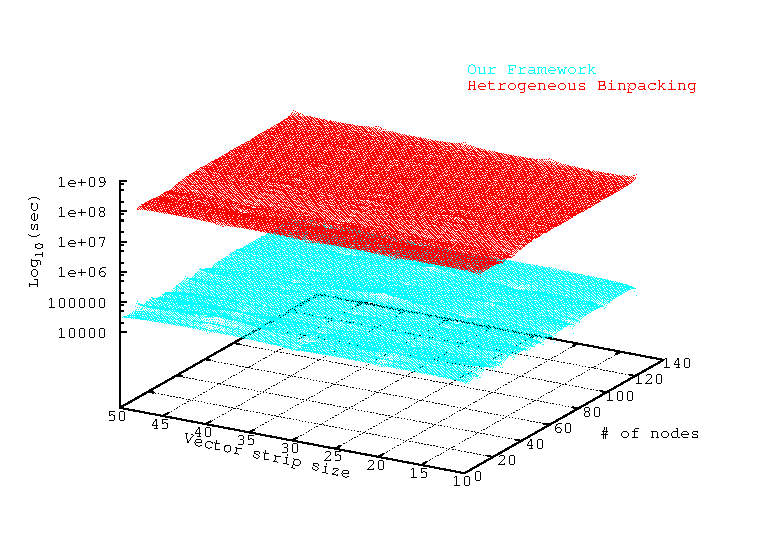
\includegraphics[angle=0, scale=0.72]{./figures/bin_surface}
    \label{fig:bin1ho}
  }
  \subfigure[2 Dimensional Convolution]{
    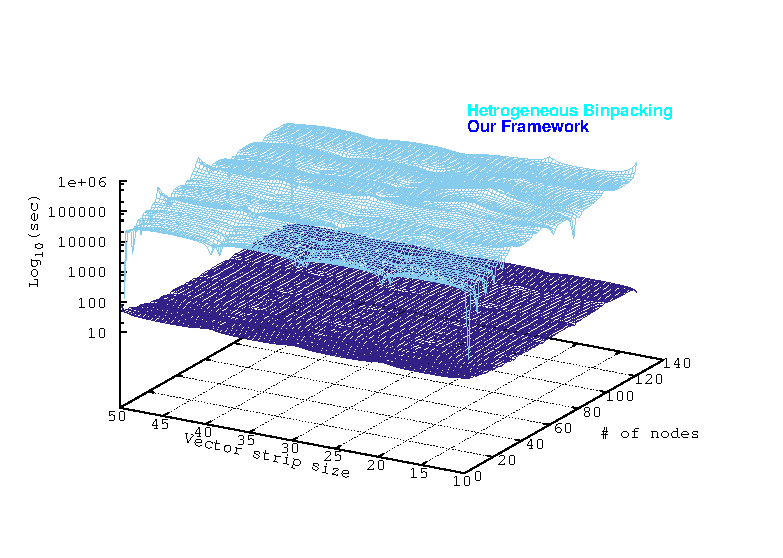
\includegraphics[angle=0, scale=0.72]{./figures/conv_surface}
    \label{fig:conv1ho}
  }
  \subfigure[Gram schmidtt linear-algebra kernel]{
    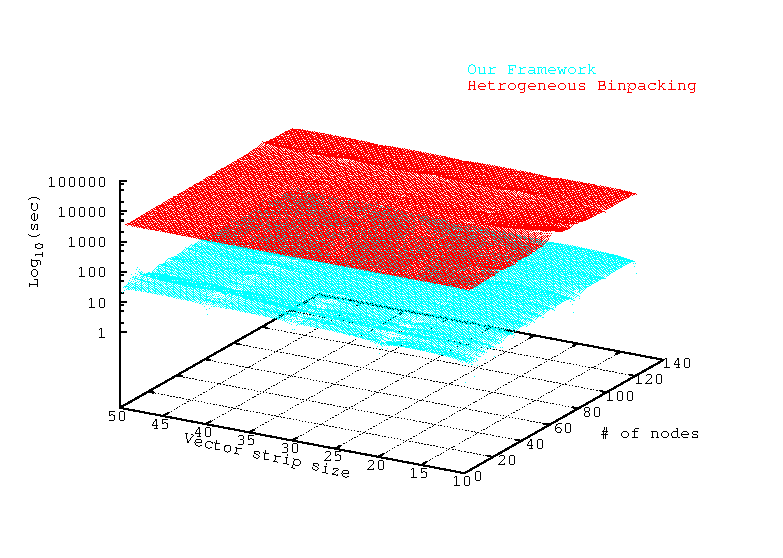
\includegraphics[angle=0, scale=0.72]{./figures/gram_surface}
    \label{fig:gram1ho}
  }
  \subfigure[2 Dimensional Seildel stencil computation]{
    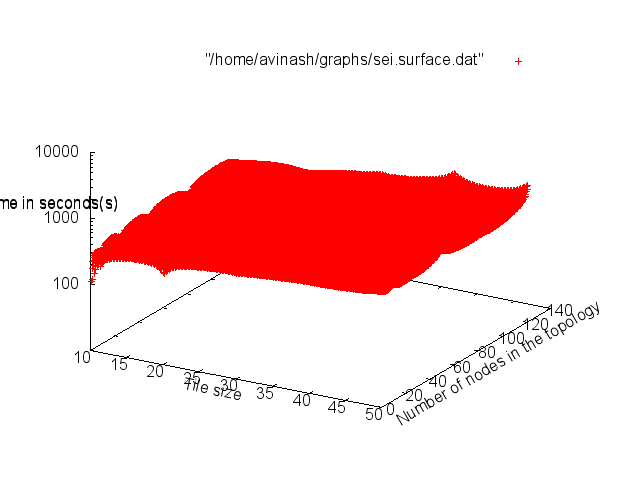
\includegraphics[angle=0, scale=0.72]{./figures/sei_surface}
    \label{fig:sei1ho}
  }
  \subfigure[2 Dimensional Jacobi stencil computation]{
    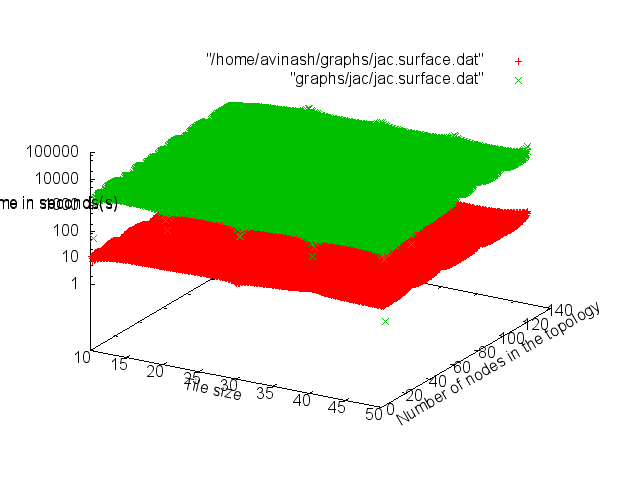
\includegraphics[angle=0, scale=0.72]{./figures/jac_surface}
    \label{fig:jacl1ho}
  }
  \caption{Comparison of execution times of ``Our Framework" and
    ``Heterogeneous Bin Packing"}
  \label{fig:ho}
\end{figure*}

\subsection{The results}
\label{sec:results-1}

The results for the experiments with the above experimental setup
comparing our approach with the aforementioned heterogeneous bin packing
approach is shown in Figure~\ref{fig:ho}. Our approach performs better
compared to heterogeneous bin packing for all the applications. The
graphs in Figure~\ref{fig:ho} consists of two surfaces layered on top of
each other. In these graphs the larger the value, the worse the latency
and hence the performance of the application. For all graphs, the
surface representing the heterogeneous bin-packing solution is always
layered atop our results, which clearly show the superiority of our
approach. Note that the z-axis in all the graph in Figure~\ref{fig:ho}
are in logarithmic scale with a base of 10. This in turn implies that
our results are almost an order of magnitude better than those obtained
by the heterogeneous bin packing heuristic.

For seidel, the results for bin-packing could not be obtained, because
the required vector element length was larger than the available
capability of the underlying hardware. Our approach is able to deal with
such a situation, by fitting the required vector length to the
capability and then running the rest in an iterative manner.

The major differences between the two algorithms are provided in
Table~\ref{tab:2}. The \textbf{Max latency} and \texttt{Min latency}
columns give the maximum and the minimum latencies for bin packing and
our framework, respectively. The final column gives the number of data
points that our framework is better compared to heterogeneous bin
packing. As we can see from Table~\ref{tab:2}, our framework out
performs the heterogeneous bin-packing on all the applications.

\begin{table*}[t!]
  \centering
  \begin{tabular}{|c|c|c|c|c|c|}
    \hline
    \textbf{Application} &
    \multicolumn{2}{|c|}{\textbf{Max latency (s)}} &
    \multicolumn{2}{|c|}{\textbf{Min latency (s)}} &
    \textbf{Better (\%)} \\
    \hline
    & {HBP} & {Our framework} &
    {HBP} & {Our framework} & HBP vs Our framework\\
    \hline
    Binomial option pricing & $1.35e+8$ & $5.27e+7$ & 77356.9 & 1 & 100 \\
    \hline
    Convolution & 489065 & 78.52 & 53.64 & 16.26 & 94\\
    \hline
    Gram Schmidt & 18984.5 & 177.97 & 2947.65 & 1.20 & 94\\
    \hline
    Gauss-Seidel & N/A & 3635.62 & N/A & 9.67 & 100\\
    \hline
    Jacobi & 13919.2 & 39.89 & 1.69 & 0.97 & 92\\
    \hline
  \end{tabular}
  \caption{Major statistics comparing heterogeneous bin packing and our framework}
  \label{tab:2}
\end{table*}

There are a number of reasons for the large differences seen in
Figure~\ref{fig:ho}.

\begin{itemize}

\item The bin packing solution gives priority to volume, which makes
  means vectors are packed into a single large vector processor, while
  giving very little consideration to the instruction count requirement.

\item The bin packing heuristic does not consider placing data-stores in
  the correct locations, in fact data-stores do not play a part in the
  whole process at all and the same can be said about communication.

\end{itemize}

Since communication does not play a part in the heuristic bin-packing
solution, we ignored the communication values when comparing with bin
packing. But, in order to show how communication can have a significant
affect onto the application design and parallelism potential in the next
section we perform design space exploration with exploration of affect
of communication as the main objective.

\subsection{Architecture exploration with communication}
\label{sec:arch-expl-with}

More results comparing the difference when communication is changed, etc.

\begin{figure*}[t!]
  \centering
  \subfigure[Binomial Option Pricing]{
    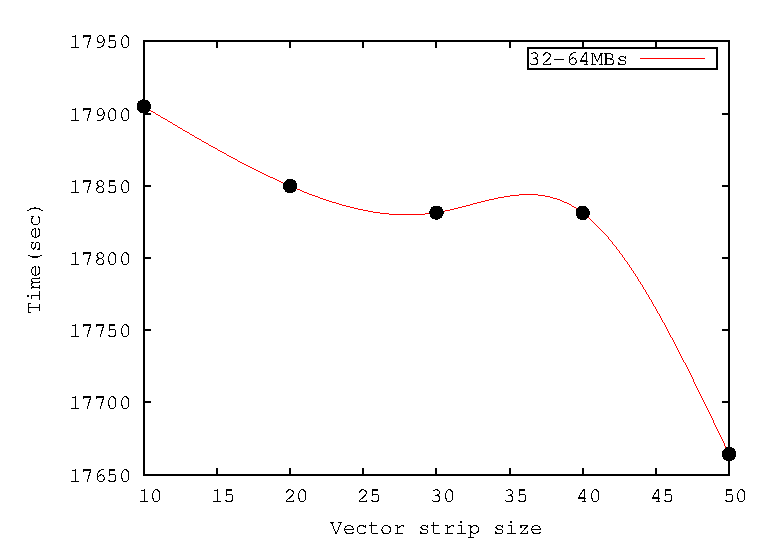
\includegraphics[angle=0, scale=0.65]{./figures/bin_32-64_surface}
    \label{fig:bin1comm}
  }
  \subfigure[2 Dimensional Jacobi stencil computation]{
    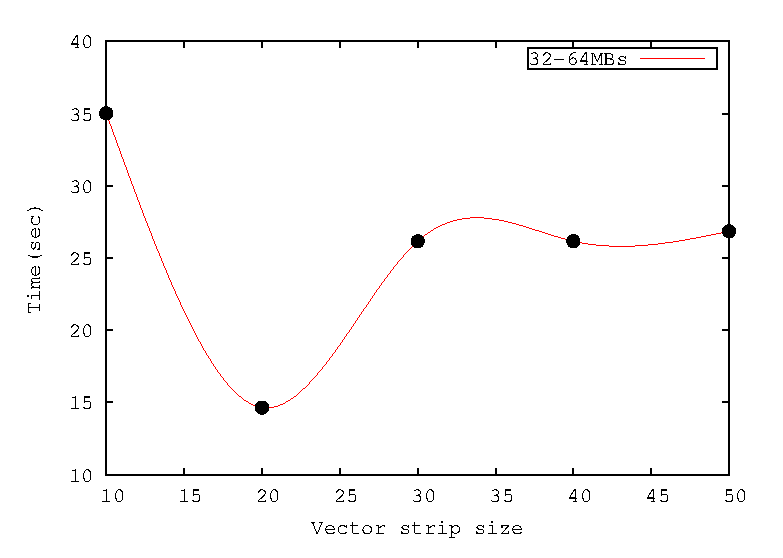
\includegraphics[angle=0, scale=0.65]{./figures/jac_32-64_surface}
    \label{fig:jac1comm}
  }
  \label{fig:comm}
\end{figure*}


%%% Local Variables:
%%% mode: latex
%%% TeX-master: "bare_conf"
%%% End:
